\chapter{Pruebas}

Con el fin de comprobar el correcto funcionamiento de la solución se realizarán distintas pruebas para corroborar que las alertas se generan correctamente y en un tiempo que pueda ser comprendido dentro de un sistema near real time. Para ello se obtendrá un conjunto de logs correctos y errores que se querrá identificar como una alerta (tanto de un error conocido con un error desconocido) con el objetivo de forzar una alerta y así comprobar que se recibe dentro del margen temporal esperado.

Debido a esto será necesario un trabajo previo de separación de logs en operaciones con errores y operaciones con funcionamiento correcto. Esto se llevará a cabo con un script Python, que separará en ficheros los dos tipos de operaciones a partir de logs producidos en un entorno de desarrollo de la aplicación. Una vez realizada la separación se podrá replicar el comportamiento de la aplicación a monitorizar, para lo que se desarrollará otro script Python que permita la publicación de logs en Kafka que reciba como entrada la cantidad de operaciones que se publican por segundo, el número de operaciones correctas que se publicarán hasta que se envíe el error y el tipo de error (conocido o desconocido). Con esto conseguimos proporcionar el estado de alarma bajo demanda y así poder comprobar la respuesta en distintas situaciones. Por otro lado se desarrollará otro script que funcione como productor de la ingesta inicial de datos.

También interesa medir si se la información obtenida de aplicar la detección de anomalías sobre la traza de logs de errores desconocidos se considere útil. Para ello una vez obtenida la alerta en el informe generado deberá estar resaltado aquellas líneas de log que en un trabajo previo se han clasificado como las que contienen la causa de la incidencia.`

\subsection{Pruebas de Alertas y Rendimiento}

Para comprobar que las alertas aportan una ayuda y mejora al sistema real, se deberá probar que efectivamente se generan las alertas y se definirá un máximo de tiempo desde que se produce la incidencia hasta que el sistema la notifica. Se ha de tener en cuenta que se está trabajando sobre un prototipo que no corre sobre un sistema en producción. Debido a la menor capacidad de computo se generarán un número inferior de logs por segundo que el sistema real y se esperarán tiempos inferiores a 5 minutos entre el registro de la incidencia en los logs y la recepción del correo con la alerta. Se probarán distintos números de logs generados por segundo que sirva de estimación de comportamiento en el sistema real, así como distintos números de reglas de alertas desplegadas.

Con la realización de las pruebas se intentará conseguir tres objetivos:

\begin{itemize}


	\item \textbf{Ejecución correcta}: Se deberá comprobar que efectivamente se genera una alerta cuando se produce una incidencia en el sistema. Para que esto se considere correcto deberá generarse siempre una alerta en cada uno de los casos de prueba propuestos.

	\item \textbf{Obtención de la alerta en Near Real Time}: en caso de que el primer punto se valide correctamente, también se ha de comprobar el tiempo que transcurre desde que se genera la incidencia (en este caso mockeandola) hasta que la alerta es recibida es inferior al tiempo estimado.

	\item \textbf{Medida de recursos utilizados}: ya que los distintos componentes de la solución estarán desplegados en docker se deberá comprobar como afecta una escalada en el las cantidades de logs a analizar con el fin de estimar que recursos serían necesarios para poder tratar con el sistema real. Se tomará de medida el uso de CPU y memoria.

\end{itemize}

Para cada una de las pruebas con distintos número de reglas desplegadas se realizará el siguiente procedimiento:

\begin{enumerate}
	\item Despliegue de los contenedores Docker con la configuración y sin datos cargados.
	\item Para cada fila de la tabla se realiza la ingesta inicial de los datos   hasta el tamaño deseado ejecución del script que genera la alarma para distintos números de entradas por segundo.
	\item Registro de tiempos de respuesta y de recursos utilizados en los contenedores.
	\item Parado y borrado de los dockers con el fin de utilizar una instancia nueva en cada prueba.
\end{enumerate}

Para registrar las pruebas se seguirá un esquema de tabla especificando el estado de la aplicación a la hora de provocarse  la incidencia, la salida el tiempo empleado y los recursos utilizados.

Con el fin de comprobar como afecta el número de reglas que se tengan desplegadas se repetirán las pruebas con un número distinto y así establecer una aproximación de los recursos utilizados con varias pruebas. Además para facilitar el proceso durante las pruebas se establecerá que las alertas se ejecutan cuando se encuentre el primer error especificando con los parámetros:

\begin{verbatim}

# (Required, frequency specific)
# Alert when this many documents matching the query occur within a timeframe
num_events: 1

# (Required, frequency specific)
# num_events must occur within this amount of time to trigger an alert
timeframe:
    hours: 1
    
\end{verbatim}

Pruebas con \textbf{una} regla desplegada:

\begin{table}[H]
\begin{tabular}{|l|l|l|l|l|}
\hline
\rowcolor[HTML]{ECF4FF} 
{\color[HTML]{000000} \textbf{Tam logs cargados en ELK}} & {\color[HTML]{000000} \textbf{Num. logs/segundo}} & {\color[HTML]{000000} \textbf{Alerta}} & {\color[HTML]{000000} \textbf{Tiempo}} & {\color[HTML]{000000} \textbf{Recursos}} \\ \hline
                                                         & 10 entrada/segundo                                &                                        &                                        &                                                 \\ \cline{2-5} 
                                                         & 50 entradas/segundo                               &                                        &                                        &                                                 \\ \cline{2-5} 
\multirow{-3}{*}{10 MB}                                  & 100 entradas/segundo                              &                                        &                                        &                                                 \\ \hline
                                                         & 10 entrada/segundo                                &                                        &                                        &                                                 \\ \cline{2-5} 
                                                         & 50 entradas/segundo                               &                                        &                                        &                                                 \\ \cline{2-5} 
\multirow{-3}{*}{50 MB}                                  & 100 entradas/segundo                              &                                        &                                        &                                                 \\ \hline
                                                         & 10 entradas/segundo                               &                                        &                                        &                                                 \\ \cline{2-5} 
                                                         & 50 entradas/segundo                               &                                        &                                        &                                                 \\ \cline{2-5} 
\multirow{-3}{*}{100 MB}                                 & 100 entradas/segundo                              &                                        &                                        &                                                 \\ \hline
                                                         & 10 entradas/segundo                               &                                        &                                        &                                                 \\ \cline{2-5} 
                                                         & 50 entradas/segundo                               &                                        &                                        &                                                 \\ \cline{2-5} 
\multirow{-3}{*}{500 MB}                                 & 100 entradas/segundo                              &                                        &                                        &                                                 \\ \hline
                                                         & 10 entradas/segundo                               &                                        &                                        &                                                 \\ \cline{2-5} 
                                                         & 50 entradas/segundo                               &                                        &                                        &                                                 \\ \cline{2-5} 
\multirow{-3}{*}{1 GB}                                   & 100 entradas/segundo                              &                                        &                                        &                                                 \\ \hline
\end{tabular}
\end{table}


Pruebas con \textbf{cinco} reglas desplegadas:

\begin{table}[H]
\begin{tabular}{|l|l|l|l|l|}
\hline
\rowcolor[HTML]{ECF4FF} 
{\color[HTML]{000000} \textbf{Tam logs cargados en ELK}} & {\color[HTML]{000000} \textbf{Num. logs/segundo}} & {\color[HTML]{000000} \textbf{Alerta}} & {\color[HTML]{000000} \textbf{Tiempo}} & {\color[HTML]{000000} \textbf{Recursos}} \\ \hline
                                                         & 10 entrada/segundo                                &                                        &                                        &                                                 \\ \cline{2-5} 
                                                         & 50 entradas/segundo                               &                                        &                                        &                                                 \\ \cline{2-5} 
\multirow{-3}{*}{10 MB}                                  & 100 entradas/segundo                              &                                        &                                        &                                                 \\ \hline
                                                         & 10 entrada/segundo                                &                                        &                                        &                                                 \\ \cline{2-5} 
                                                         & 50 entradas/segundo                               &                                        &                                        &                                                 \\ \cline{2-5} 
\multirow{-3}{*}{50 MB}                                  & 100 entradas/segundo                              &                                        &                                        &                                                 \\ \hline
                                                         & 10 entradas/segundo                               &                                        &                                        &                                                 \\ \cline{2-5} 
                                                         & 50 entradas/segundo                               &                                        &                                        &                                                 \\ \cline{2-5} 
\multirow{-3}{*}{100 MB}                                 & 100 entradas/segundo                              &                                        &                                        &                                                 \\ \hline
                                                         & 10 entradas/segundo                               &                                        &                                        &                                                 \\ \cline{2-5} 
                                                         & 50 entradas/segundo                               &                                        &                                        &                                                 \\ \cline{2-5} 
\multirow{-3}{*}{500 MB}                                 & 100 entradas/segundo                              &                                        &                                        &                                                 \\ \hline
                                                         & 10 entradas/segundo                               &                                        &                                        &                                                 \\ \cline{2-5} 
                                                         & 50 entradas/segundo                               &                                        &                                        &                                                 \\ \cline{2-5} 
\multirow{-3}{*}{1 GB}                                   & 100 entradas/segundo                              &                                        &                                        &                                                 \\ \hline
\end{tabular}
\end{table}

\subsubsection{Muestra de los datos}

--TODO--

En esta parte se mostrará una gráfica con los resultados obtenidos (Tiempo respuesta/Carga inicial) para cada uno de las distintos números de reglas.


\subsection{Pruebas del detector de anomalías en errores desconocidos}

Como objetivo secundario de la aplicación se buscará probar que para los errores desconocidos se proporciona una herramienta que pueda ayudar a la resolución de la alerta.

Para esta prueba se han buscado operaciones fallidas con un error desconocido en las que se distinguieron claramente la causa del error. En este caso varias operaciones en las que se produjo una excepción java no controlada que llegó a registrarse.

Por otro lado, se realizará un entrenamiento inicial del modelo utilizando un conjunto logs de resultados correctos de la operación a probar. Para ello se utilizarán los logs utilizados en las pruebas de rendimiento y se filtrarán por operaciones para entrenar un modelo por operación. Una vez entrenados los modelos y aplicada la detección de anomalías se genera un informe que resalte aquellas líneas que difieran de las líneas base. 

Se definirá como correcto los casos en los que se diferencien aquellas líneas que en un trabajo previo se clasifiquen como las que aportan información para tratar la incidencia, es decir, las líneas que se consideren anómalas. El ejemplo de salida es el siguiente:

\begin{figure}[H]
\centerline{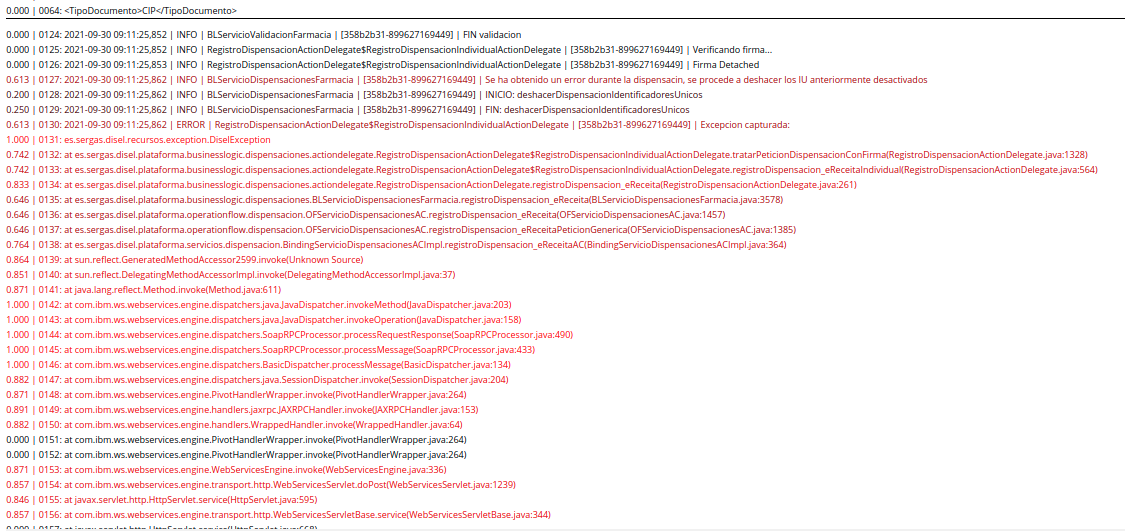
\includegraphics[width=15cm]{figuras/report.png}}
\caption{Ejemplo salida detección anomalías}
\label{enlace1}
\end{figure}




El resultado se considera correcto, ya que se efectivamente las líneas causantes del problema se resaltan como anomalías, sin embargo, no es un resultado perfecto, ya que también se están considerando anomalías (aunque con un valor de diferencia menor) debido al gran número de caminos y posibilidades posibles en las operaciones. Sin embargo, se considera que el resultado es lo suficientemente correcto, se espera que la salida pueda ayudar a personal no técnico encargado de la monitorización a facilitar el trabajo de revisión y búsqueda y con los resultados obtenidos se cumple esta condición.


